\newpage
\section*{Figure Captions}
\mt{captions are limited to 150 words}


\begin{flushleft}

%==================
% FIGURE 1
%% 175 words
\textbf{Figure \ref{fig:diagram}:}
	The parameters of a correlative metamodel model (left column) are conditioned on the predictions of a mechanistic sub-model (right column).
	The metamodel ($\theta_M$) operates at a single ecological scale and uses occurrence data (\(X_M\)) and explanatory variables ($D_M$) to produce a naive (i.e., not conditioned on sub-models) prediction $\psi_N$.
	The mechanistic sub-model \(\theta_S\) includes data about the response (\(X_S\)) of lower-level behaviours of the system to explanatory variables ($D_S$). 
	The models are integrated by calibrating $\theta_M$ to data ($X_M, D_M$) as well as the output of the sub-model ($\psi_S$). 
	This is possible because predictions from the sub-model ($\psi_S$) emerge at the scale of the metamodel via a scaling function \(g(\theta_S, D_S)\).
	The final prediction can be obtained by applying the integrated model to the original explanatory variables (as shown) or, if projection is desired, on some new set of explanatory variables (e.g., future climate).
	This prediction incorporates multiple sources of information coming from several calibration datasets (i.e., $X_M, D_M, X_S, $ and $D_S$) as well as from multiple types of models (i.e., $\theta_M$ and $\theta_S$).


%==================
% FIGURE 2
%% 88 words
\textbf{Figure \ref{fig:ex1_sampling}:}
	Two simulated data sets used to illustrate the model integration framework.
	(a) Presences (circles) or absences (x's) of the species in ecological space, where precipitation ranges from 0--1.
	(b) Growth rate ($r$) as a function of manipulations to the precipitation regime (whiskers show $\pm$ 1 SE), with a larger range for precipitation (i.e., \(-\)1--1).
	The dashed line shows the threshold above which the species net growth rate is positive (implying presence).
	Axis scales for temperature and precipitation are arbitrary, but note the different scales on the horizontal axes.
	
%==================
% FIGURE 3
%%  120 words
\textbf{Figure \ref{fig:ex1_precip}:}
	Results of integration showing the probability of presence (\(\psi\)) when considering only precipitation.
	(a) Naive model, using only presence-absence data. Uncertainty increases dramatically when attempting to project beyond the scope of the source data (represented by the horizontal line above the bottom axis).
	(b) Mechanistic model, using observations of an experiment to infer probability of presence. Predictions are highly precise due to high quality source data, but are likely to be overly optimistic given the simplicity in assuming only precipitation determines probability of presence (see text).
	(c) Integrated model, showing predictions that are intermediate between the two sub-models and uncertainty that is reduced compared to (a).
	Uncertainty is represented as dashed lines, showing the limits of 90\% Bayesian credible intervals.

%==================
% FIGURE 4
%% 75 words
\textbf{Figure \ref{fig:ex1_map}:}
	Maps showing the predicted probability of presence (\(\psi\); (a) and (c)) and the standard deviation of \(\psi\) ((b) and (d)) for the naive and integrated models.
	Historical (e.g., where presence-absence samples were available) and predicted future precipitation regimes are shown below the horizontal axes.
	Uncertainty in the naive model was extreme when predicting beyond the historical precipitation regime.
	Uncertainty in the integrated model was considerably reduced, reflecting the additional information provided by the mechanistic model.


%==================
% FIGURE 5
%% 133 words
\textbf{Figure \ref{fig:ex2}:}
	Results of model integration for sugar maple, \emph{Acer saccharum}.
	The mechanistic sub-model Phenofit predicts present (A) and future (B) suitability using phenological information, but does not provide estimates of uncertainty.
	Predictions from a naive metal-model for the present (C) were quite similar to the sub-model, but future predictions (D) were somewhat different, and uncertainty was extreme at the predicted range margins for both present (E) and future (F).
	Applying the integration results in reduced suitability overall, possibly due to overfitting regions where the models disagree, but patterns in relative suitability largely reflected information from both models for both present (G) and future (H) climate.
	Integrated model uncertainty for both present (I) and future (J) climates is reduced near range margins but slightly increased in areas where uncertainty was low in the naive model.
	

%==================
% FIGURE 6
%% 65 words
\textbf{Figure \ref{fig:management}:}
	Sample workflow for applying the models presented in the first example in a management context.
	Critical steps include specifying the metamodel, identifying additional sources of information to be used as constraints on the metamodel, and using the integrated prediction for decision-making.
	As additional information becomes available from monitoring the results of management, this information can be incorporated in additional sub-models to further refine the metamodel.


\end{flushleft}

%==================
% FIGURE 1

\newpage
\begin{figure}[p!]


%\documentclass{article}
%\usepackage{tikz}
%\usepackage{tikz-cd}
%\usepackage{amsmath}

%\usetikzlibrary{calc, shapes}
%\usetikzlibrary{shapes.geometric,shapes.arrows,decorations.pathmorphing}
%\usetikzlibrary{matrix,chains,scopes,positioning,arrows,fit}
%\begin{document}

%% --------------------------------------------------------------------------------------
%% ------part 1--------------------------------------------------------------------------
%% --------------------------------------------------------------------------------------

\begin{tikzpicture}
	
\matrix(m) [matrix of nodes, column sep=-0.5em,
	row sep=2em,
	minimum width=4em,
	minimum height=2em,
	column 1/.style={anchor=west, align=left, text width=10em},
	multi/.style={rectangle split,rectangle split parts=2}]
	{
	% zeroth line
	% blank space 
	&
	\textbf{Correlative Metamodel}
	&
	&
	\textbf{Mechanistic sub-model}
	\\
	% first line
	Data % m 1-1
	&
	$X_{M}, D_{M}$ % m 1-2
	&
	&
	$X_{S}, D_{S}$ % m 1-4
	\\
%second line
	|[multi]| Process % m 2-1 
	\nodepart{second}
	(prior and likelihood)
	&
	|[multi]|$p(\theta_{M})$ % m 2-2
	\nodepart{second}
	$p(X_{M} \mid \theta_{M}, D_{M})$
	&
	&
	|[multi]|$p(\theta_{S})$
	\nodepart{second}
	$p(X_{S} \mid \theta_{S}, D_{S})$
	\\

%third line
	
	Posterior
	&
	$p(\theta_{M} \mid X_{M}, D_{M})$
	&
	&
	$p(\theta_{S} \mid X_{S}, D_{S})$
	\\

%fourth line
	Prediction
	&
	$\psi_N = f(\theta_M, D_M)$
	&
	&
	$\psi_S = g(\theta_S, X_S, D_S)$
	\\

%fifth line
	Data
	&
	&
	&
	$\psi_S$
	\\
%sixth line
	|[multi]| Process
	\nodepart{second}
	(integrated likelihood)
	&
	$p(\theta_M \mid X_M, D_M)$
	&
	&
	$p(\psi_S \mid \theta_M)$
	\\


%seventh line
	Integrated posterior
	&
	&
	$p(\theta_M \mid \psi_S, X_M, D_M)$
	&
	\\

%eighth line
	Integrated prediction
	&
	&
	$\psi_I = f(\theta_M, D_M)$
	&
	\\
}; %end matrix

% The names of the nodes are automatically generated in the previous matrix. Since the
% matrix was named ``m'', all nodes have the name m-row-column

% metamodel
\draw [->] (m-2-2.south) -- (m-3-2.north);
\draw [->] (m-3-2.south) -- (m-4-2.north);
\draw [->] (m-4-2.south) -- (m-5-2.north);

%%mechanistic model
\draw [->] (m-2-4.south) -- (m-3-4.north);
\draw [->] (m-3-4.south) -- (m-4-4.north);
\draw [->] (m-4-4.south) -- (m-5-4.north);

%%separation line
\draw [line cap=rect, transform canvas={yshift=-1em}] (m-5-1.south west) -- (m-5-4.south east);
%(\linewidth-\pgflinewidth,0); 

\tikzstyle{opt}=[gray,dashed,rounded corners];
\draw [->,style=opt] (m-4-2.west) to[bend right=50] (m-7-2.west);
\draw [->,style=opt] (m-5-4.south) to (m-6-4.north);

%%integrated model
\draw [->] (m-7-2.south) -- (m-8-3.north west);
\draw [->] (m-6-4.south) -- (m-7-4.north);
\draw [->] (m-7-4.south) -- (m-8-3.north east);
\draw [->] (m-8-3.south) -- (m-9-3.north);


\end{tikzpicture}


\caption{}
\label{fig:diagram}
\end{figure}


%==================
% FIGURE 2
\newpage
\begin{figure}[p!]
	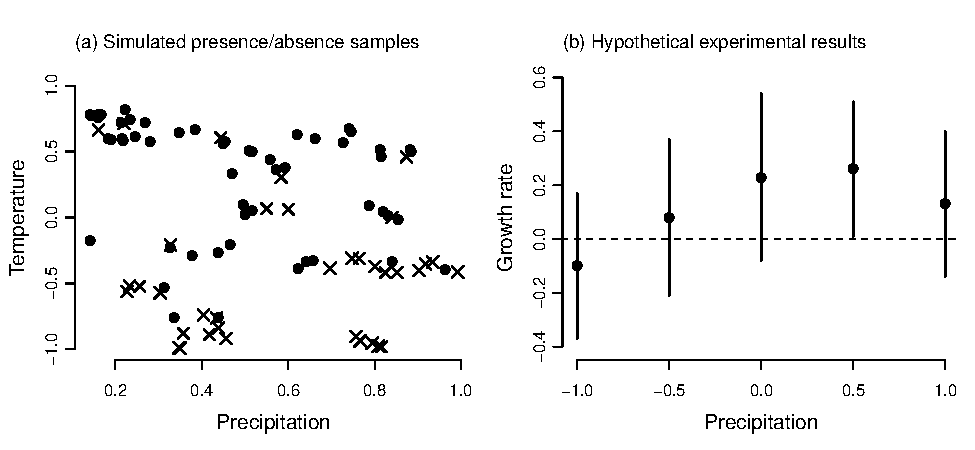
\includegraphics{ex1_sampling.pdf}
	\caption{}
	\label{fig:ex1_sampling}
\end{figure}


%==================
% FIGURE 3
\newpage
\begin{figure}[p!]
	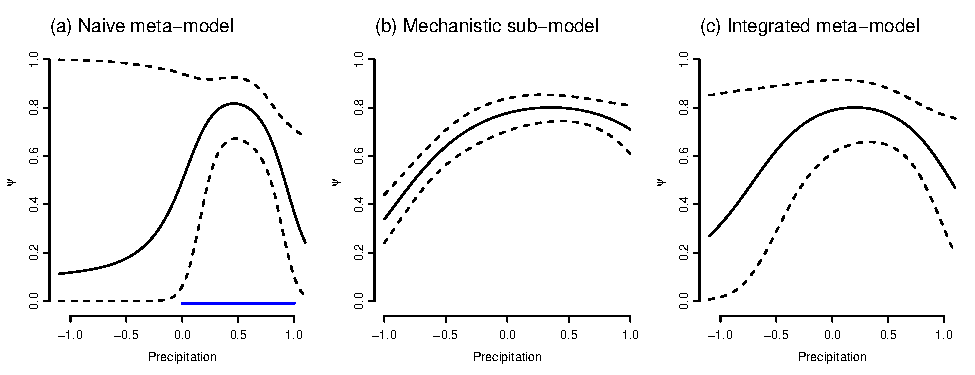
\includegraphics{ex1_precip.pdf}
	\caption{}
	\label{fig:ex1_precip}
\end{figure}


%==================
% FIGURE 4
\newpage
\begin{figure}[p!]
	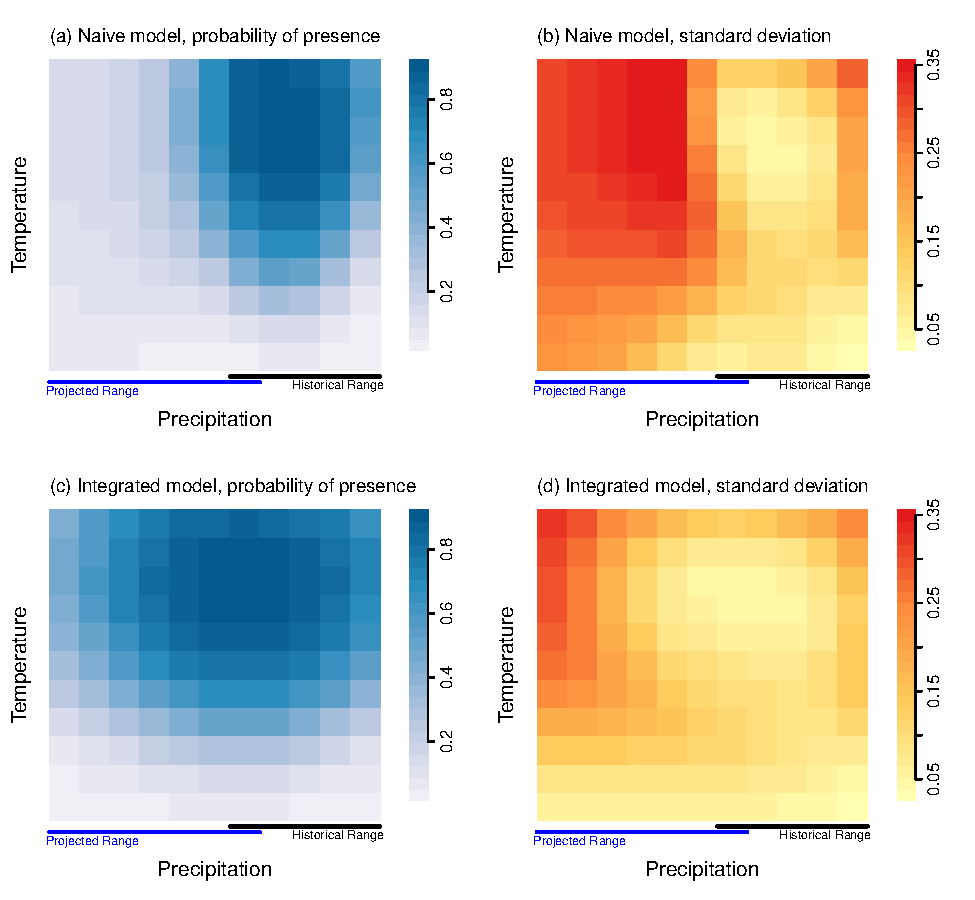
\includegraphics[width=5.25in]{ex1_map.pdf}
	\caption{}
	\label{fig:ex1_map}
\end{figure}


%==================
% FIGURE 5
\newpage
\begin{figure}[p!]
	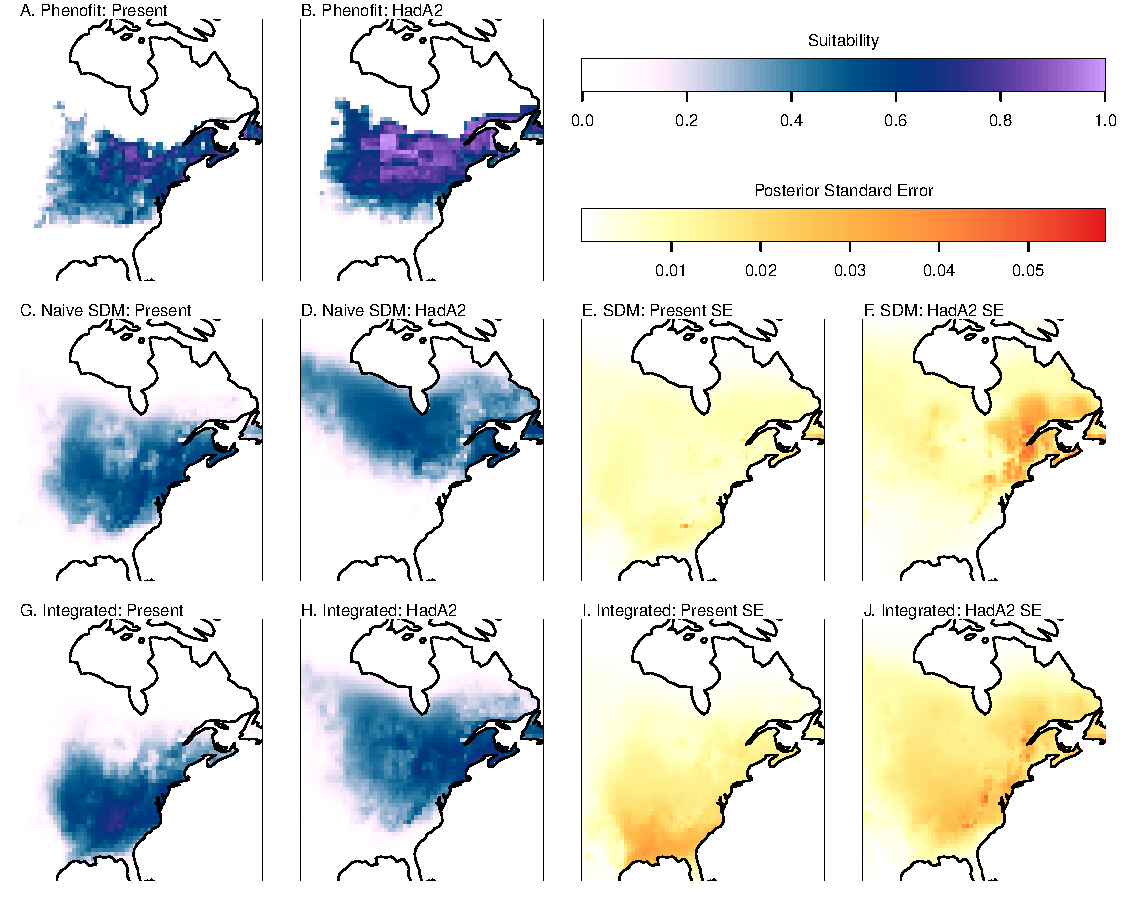
\includegraphics[width=6in]{ex2.pdf}
	\caption{}
	\label{fig:ex2}
\end{figure}


%==================
% FIGURE 6
\newpage
\dm{Could write out the word Objectives in the Figure}
\aa{The box in the right could maybe just say: monitoring of management actions}
\begin{figure}[p!]
	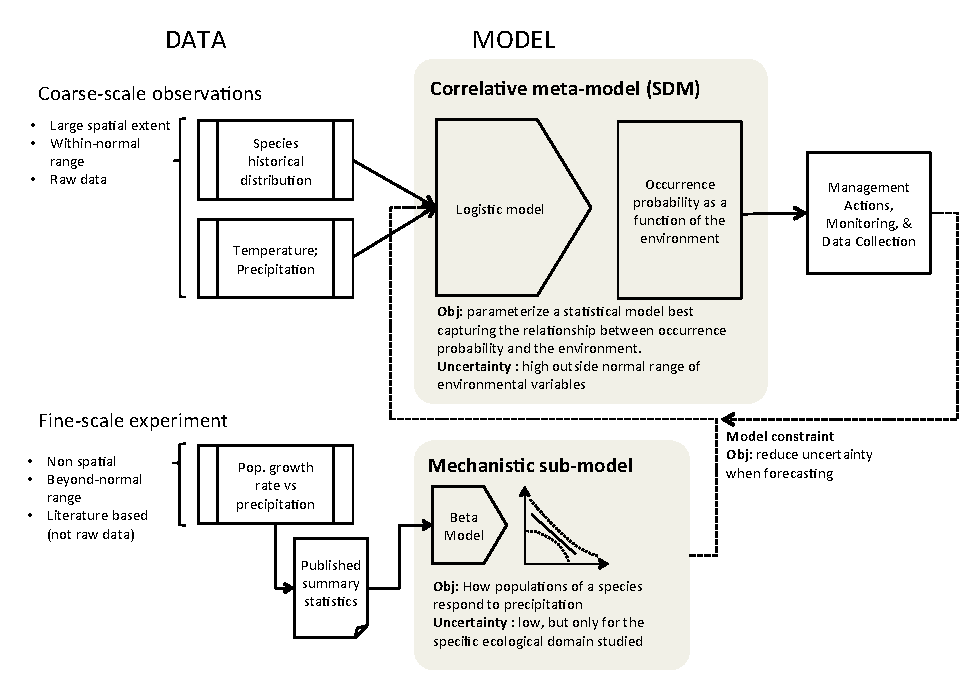
\includegraphics{management.pdf}
	\caption{}
	\label{fig:management}
\end{figure}
